\section{Numerical integration}

Consider evaluating the definite integral 
\[\int_a^bf(x)\,dx.\]

For the vast majority of function, the antiderivataive is not known. For example, we can't find:
\[\int\sqrt{1+x^3}\,dx\quad \text{or}\quad \int e^{x^2}\,dx.\]

When applying integration to a real application this is a problem.

When an impossible integral is encountered, we must use a \textbf{numerical method} to approximate the answer.

\subsection{Trapezium method}
We want to estimate the integral of $f(x)$ on the interval $[a,b]$, which represents the area under the curve $y=f(x)$ from $a$ to $b$.

\begin{figure}[H]
\centering
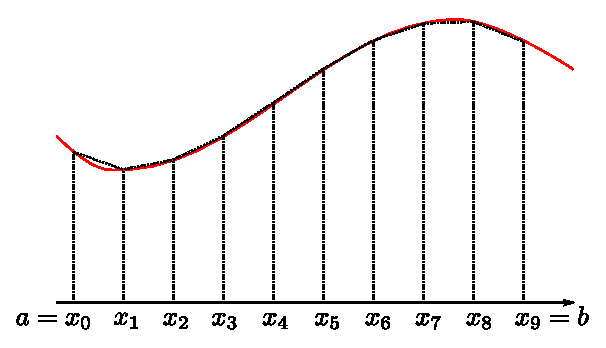
\includegraphics[scale=0.7]{img/trapezium-rule-integration}
\caption{Forming trapeziums with height of the sides dictated by the curve $y=f(x)$ over the interval $[a,b]$.}
\label{fig:trapezium-rule-integration}
\end{figure}

We choose $n$ number of pieces. Divide the interval $a\le x\le b$ into $n$ (equal) pieces with points
\[a=x_0<x_1<x_2<\dots<x_{n-1}<x_n=b.\]
On each piece of the interval, we build a trapezium by joining points on the curve by a straight line. We calculate the total area by summing all the area of the trapezia. This is our estimate of the integral.

To start with, let $h$ be the width of one piece of the interval, i.e.
\[h=\frac{b-a}{n},\]
then we have
\[x_k=x_0+kh,\quad k=0,1,2,\dots,n.\quad x_0=a,\quad x_n=b.\]

Let us consider the trapezium based on the piece $[x_{k-1},x_k]$, whose width is $h$. The height of the sides of the trapezium are $f(x_{k-1})$ and $f(x_k)$. So the area is
\[h\frac{f(x_{k-1})+ f(x_k)}{2}.\]

\begin{figure}[H]
\centering
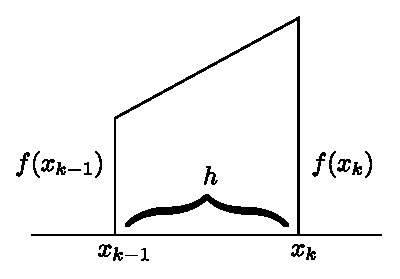
\includegraphics[scale=0.7]{img/one-trapezium}
\captionstyle{\centering\it}
\caption{Trapezium constructed over each piece of the interval, where each piece has width $h$.}
\label{fig:one-trapezium}
\end{figure}

Then the total area under the curve over $[a,b]$ is the sum:
\begin{eqnarray*}
\text{Area}&=&h\frac{f(x_{0})+ f(x_1)}{2}+h\frac{f(x_{1})+ f(x_2)}{2}+\dots+h\frac{f(x_{n-1})+ f(x_n)}{2} \\
&=&\frac{h}{2}\left[(f(x_0)+f(x_1))+(f(x_1)+f(x_2))+\dots+(f(x_{n-1})+f(x_n))\right] \\
&=& \frac{h}{2}\left[f(x_0)+2(f(x_1)+f(x_2)+\dots+f(x_{n-1}))+f(x_n)\right] \\
&=&\frac{h}{2}\left[f(x_0)+2\sum_{k=1}^{n-1}f(x_k) +f(x_n)\right].
\end{eqnarray*}

We can think of the sum as follows, we have the two outer sides of the first and last trapezium, then every trapezium in-between shares its sides with its neighbour, therefore we require two lots of the interior sides.

\begin{example}
Using the trapezium method, estimate
\[\int_0^1\frac{1}{1+x^4}\,dx.\]
We choose $n=4$, then
\[h=\frac{1-0}{4}=\frac{1}{4},\quad x_k=kh,\quad k=0,1,2,3,4.\]
Also, note that
\[f(x)=\frac{1}{1+x^4},\quad \text{i.e.}\quad f(x_k)=\frac{1}{1+x_k^4}.\]
Therefore, we have
\begin{eqnarray*}
\int_0^1\frac{1}{1+x^4}\,dx&\approx&\frac{h}{2}\left[f(x_0)+2(f(x_1)+f(x_2)+f(x_3))+f(x_4)\right] \\
&=&\frac{1}{8}\left[f(0)+2(f\left(\frac{1}{4}\right)+f\left(\frac{1}{2}\right)+f\left(\frac{3}{4}\right))+f(1)\right]\\
&=&\frac{1}{8}\left[1+2\left(\frac{256}{257}+\frac{16}{17}+\frac{256}{337}\right)+\frac{1}{2}\right]\\
&=&0.862.
\end{eqnarray*}

\begin{figure}[H]
\centering
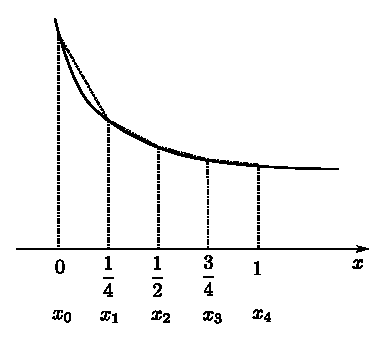
\includegraphics[scale=0.8]{img/trapexium-rule-ex1}
\caption{Numerically integrating under $y=1/(1+x^4)$. Dividing interval into 4 pieces of width $h=1/4$.}
\label{fig:trapexium-rule-ex1}
\end{figure}

This is an over-estimate of the integral since $y=f(x)$ is convex (i.e. it curves up like a cup). If it were concave (i.e. curved down like a cap), then you would have an under-estimate. 
\end{example}
